\documentclass[12pt, openright, a4paper, brazil, oneside]{abntex2}

\usepackage{lmodern}                 
\usepackage[T1]{fontenc}             
\usepackage[utf8]{inputenc}    
\usepackage[alf]{abntex2cite}     
\usepackage[brazil]{babel}           
\usepackage{amsmath, amsfonts, amssymb, amsthm} 
\usepackage{graphicx}                
\usepackage{microtype}              
\usepackage{indentfirst}             
\usepackage{color}                   
\usepackage{hyperref} 
\usepackage{fancyhdr}        
\usepackage{tabularx}
\usepackage{amsmath}
\usepackage{booktabs} 
\usepackage{array}
\usepackage[top=3cm,left=3cm,right=2cm,bottom=2cm]{geometry}
\graphicspath{{figuras/}}

\pagestyle{fancy}
\fancyhf{} 
\fancyfoot[C]{\thepage} 

% Configurações de aparência do PDF final
\hypersetup{
    pdftitle={UTILIZAÇÃO DE REDES NEURAIS NA ANÁLISE E PREVISÃO DA TEMPERATURA MÉDIA EM ITAPETINGA-BA}, 
    pdfauthor={Lucas Silva de Oliveira},
    pdfsubject={Trabalho de Conclusão de Curso},
    pdfcreator={LaTeX with abnTeX2},
    pdfkeywords={redes neurais}{análise de séries temporais}{meteorologia},
    colorlinks=true,                
    linkcolor=black,                 
    citecolor=black,                
    filecolor=magenta,             
    urlcolor=black,
    breaklinks=true
}

% \bibliographystyle{abntex2-alf}

% Documento
\begin{document}

    % Capa
    \begin{capa}
        \center
        
\includegraphics[width=2cm]{template/ifbaiano.png}\\[0.2cm]
        {\ABNTEXchapterfont\LARGE INSTITUTO FEDERAL DE EDUCAÇÃO, CIÊNCIA E TECNOLOGIA BAIANO}\\[0.2cm]
        {\ABNTEXchapterfont\LARGE Bacharelado em Sistemas de Informação} \\[4cm]

        {\ABNTEXchapterfont\bfseries\LARGE UTILIZAÇÃO DE REDES NEURAIS NA ANÁLISE E PREVISÃO DA TEMPERATURA MÉDIA EM ITAPETINGA-BA}\\[4cm]

        {\ABNTEXchapterfont\large Lucas Silva de Oliveira}\\[4cm]

        \vfill
        \large Itapetinga - Bahia\\
        \today
    \end{capa}

    % Folha de rosto
    \begin{folhaderosto}

        \begin{center}
            \ABNTEXchapterfont\bfseries\LARGE UTILIZAÇÃO DE REDES NEURAIS NA ANÁLISE E PREVISÃO DA TEMPERATURA MÉDIA EM ITAPETINGA-BA
        \end{center}

        \vspace{4cm}

        \begin{center}
            {\ABNTEXchapterfont\large Lucas Silva de Oliveira}
        \end{center}

        \vspace{4cm}

        \vspace*{\fill}
        \begin{flushright}
            \begin{minipage}{8.6cm}
                Trabalho de Conclusão de Curso apresentado como 
                requisito parcial para obtenção 
                do título de Bacharel em Sistemas de Informação.
                
                \vspace{0.5cm}
                \textbf{Orientador(a)}: Prof(a). Dr(a). Nome do(a) Orientador(a).
            \end{minipage}
        \end{flushright}

        \vspace{5.5cm}

        \begin{center}
            \large Itapetinga - Bahia\\
            \today
        \end{center}

    \end{folhaderosto}

    \newpage
    \begin{center}
        \begin{center}
            \ABNTEXchapterfont\bfseries\LARGE UTILIZAÇÃO DE REDES NEURAIS NA ANÁLISE E PREVISÃO DA TEMPERATURA MÉDIA EM ITAPETINGA-BA
        \end{center}

        \vspace{3cm}

        \begin{center}
            {\ABNTEXchapterfont\large Lucas Silva de Oliveira}
        \end{center}

        \vspace{4cm}
    
        \begin{flushright}
            \begin{minipage}{8.6cm}
                Trabalho de Conclusão de Curso apresentado como 
                requisito parcial para obtenção 
                do título de Bacharel em Sistemas de Informação.
            \end{minipage}
        \end{flushright}
        

        \vspace{1cm}
        
        \begin{center}

            \textit{BANCA EXAMINADORA:}
            \vspace{2cm}

            \begin{minipage}{12cm}
                \begin{center}
                    \rule{10.5cm}{0.5pt} \\ % Linha para o Orientador
                    Prof(a). Dr(a). Nome do(a) Orientador(a) (Orientador(a)) \\ IFBAIANO \\
                    \vspace{0.5cm}
                    \rule{10.5cm}{0.5pt} \\ % Linha para o Avaliador 1
                    Prof(a). Dr(a). Nome do(a) Avaliador(a) \\ Instituição \\
                    \vspace{0.5cm}
                    \rule{10.5cm}{0.5pt} \\ % Linha para o Avaliador 2
                    Prof(a). Dr(a). Nome do(a) Avaliador(a) \\ Instituição
                \end{center}
            \end{minipage}
        \end{center}
    \end{center}

    \newpage
    % Dedicatória
    \begin{dedicatoria}
        \vspace*{\fill}
        \begin{flushright}
            \noindent
            \textit{Dedico este trabalho a\ldots}
        \end{flushright}
    \end{dedicatoria}

    % Agradecimentos
    \begin{agradecimentos}
        Agradeço a\ldots
    \end{agradecimentos}

    % Epígrafe
    \begin{epigrafe}
        \vspace*{\fill}
        \begin{flushright}
            \textit{
            "Coloca aqui a epígrafe."\\
            --- Nome do autor da epígrafe}
        \end{flushright}
    \end{epigrafe}

    % Resumo
    \begin{resumo}
        Aqui fica o resumo em português.\\   
        \textbf{Palavras-chave}: redes neurais, séries temporais, meteorologia.
    \end{resumo}

    % Abstract
    \begin{abstract}
        Aqui fica o resumo em inglês.\\ 
        \textbf{Keywords}: neural networks, time series, meteorology.
    \end{abstract}

    \newpage

    \pdfbookmark[0]{Sumário}{toc}
    \tableofcontents* 
    \thispagestyle{empty} 

    \setcounter{chapter}{0}
    \setcounter{page}{0}    

    \chapter{INTRODUÇÃO}

Aqui é onde ficara a introdução da problemática

\section{OBJETIVOS}
    O presente projeto tem como objetivo utilizar redes neurais na análise e previsão das variações meteorológicas no 
    município de Itapetinga-BA ao longo do tempo, identificando padrões sazonais, tendências de longo prazo e 
    possíveis anomalias climáticas, a fim de contribuir com o planejamento urbano, agrícola e ambiental da região.
    
    Este trabalho também contará com os seguintes objetivos específicos:

    \begin{itemize}
        %\setlength{\itemsep}{1em}
        \item Analisar as séries temporais dos dados de temperatura, precipitação e outros 
              parâmetros climáticos no município de Itapetinga-BA, utilizando redes neurais artificiais.
        \item Identificar tendências de aquecimento, variações de precipitação e outros 
              impactos ambientais na cidade, por meio de modelos de previsão baseados em redes neurais.
        \item Avaliar as mudanças climáticas em Itapetinga-BA, comparando as previsões 
              geradas pelas redes neurais com os dados históricos para identificar anomalias.
    \end{itemize}

\section{JUSTIFICATIVA}
    %Talvez alterar e não falar do código florestl no momento, começar falando do mundo, mudanças climáticas,brasil, bahia e previsão com redes neurais
    Suspeita-se que as mudanças ambientais e climáticas tenham como principal responsável a ação humana, 
    impulsionada pela intensa atividade industrial. A revolução industrial marcou o início dessa transformação, 
    promovendo a adoção de novas fontes de energia e o fortalecimento do consumo de combustíveis fósseis, como o 
    carvão mineral inicialmente e, posteriormente, o petróleo~\cite{mendoncca2006aquecimento}.
    
    À vista disso, nas últimas décadas, os debates sobre as mudanças climáticas e a necessidade de uma sociedade 
    mais consciente e participativa na preservação ambiental e no desenvolvimento sustentável se tornaram cada 
    vez mais intensos. Em 1972, ao identificar a vulnerabilidade do planeta Terra, houve um esforço mundial conjunto
    em entender os problemas ambientais e ponderar medidas para previnir ou amenizar determinados crises.
    
    A Conferência das Nações Unidas para o Meio Ambiente Humano, também conhecida como Conferência de Estocolmo, 
    realizada em 1972 na cidade de Estocolmo, na Suécia, foi um marco histórico por ser a primeira conferência 
    global com foco no meio ambiente. Durante o evento, deu-se início à estruturação de mecanismos de proteção 
    ambiental, que foram ampliados na Segunda Conferência das Nações Unidas sobre o Meio Ambiente e 
    Desenvolvimento, realizada em 1992, conhecida como Rio-92. Nessas conferências, foram estabelecidos 
    diversos acordos para a proteção do meio ambiente, da biodiversidade e de outros aspectos relacionados à 
    sustentabilidade, como a Agenda 21~\cite{passos2009}.


    Entretanto, de acordo com relatório especial publicado em 2020 pelo Painel Intergovernamental sobre Mudanças Climáticas (IPCC), 
    desde o período pré-industrial, a temperatura média do ar na superfície da Terra quase dobrou em relação à média 
    global registrada anteriormente. Além disso, estima-se que 23\% das emissões antrópicas de gases de efeito estufa 
    sejam provenientes de atividades relacionadas à agricultura, silvicultura e outras práticas agrícolas.

    No Brasil, em 2019, logo após o início do mandato do governo eleito no ano anterior, as invasões às terras 
    indígenas por grupos ilegais, como garimpeiros, foram retomadas. Como resultado, a taxa de desmatamento em 
    junho daquele ano já apresentava um aumento alarmante de 60\% em relação ao mesmo mês do ano anterior. 
    Além disso, houve uma intensificação de atividades ilícitas, como a grilagem de terras, mineração clandestina 
    e exploração madeireira na Amazônia~\cite{barretto2020}.

    \citeonline{barretto2020} afirma que esse aumento foi impulsionado pelos questionamentos levantados pelo então 
    presidente da República, Jair Messias Bolsonaro, que colocava em dúvida a veracidade das informações fornecidas 
    por órgãos públicos responsáveis pelo monitoramento ambiental. Além disso, suas declarações sobre a desarticulação do sistema de 
    regulação ambiental reforçaram, entre seus apoiadores, a percepção de que havia uma espécie de "liberação total".
    Isso resultou na intensificação de práticas prejudiciais ao meio ambiente, à saúde pública e ao tecido social.

    %Falar da bahia e suas mudanças climáticas se possível
    
    %Elencar com a utilização de métodos de previsão para influenciar novas políticas públicas


\section{ORGANIZAÇÃO DOS CAPÍTULOS}
%Falar sobre como se dará os capítulos, quais são e o que cada um irá abordar.
    \chapter{FUNDAMENTAÇÃO TEÓRICA}
Neste capítulo, são apresentados os principais conceitos e fundamentos necessários para a compreensão, 
entendimento e progresso deste trabalho.

\section{Séries Temporais}
    Muitas pessoas, em algum momento, já imaginaram como seria prever o futuro e ter acesso a informações sobre eventos 
    ou situações de suas vidas. Essa curiosidade reflete um desejo universal, mas também uma necessidade presente em 
    diversas áreas, como na gestão governamental, no setor financeiro e em contextos sociais. Nesse cenário, surge o 
    conceito de Série Temporal, definido como um conjunto de observações organizadas sequencialmente no tempo, 
    representadas por \( x_t \), com cada valor correspondente a um instante específico \(t\)~\cite{box2015}. O estudo de 
    Séries Temporais permite não apenas compreender as características de fenômenos que evoluem ao longo do tempo, mas 
    também desenvolver e ajustar modelos estatísticos capazes de explicar ou prever o comportamento dos dados 
    observados.
    
    De acordo com~\citeonline{brockwell2002}, séries temporais podem ser classificadas 
    discretas e continuas, uma série temporal é discreta quando o conjunto \( t_0 \) de tempos em que as observações 
    são feitas é um conjunto discreto, como o caso de observações que são realizadas em um determinado intervalo de 
    tempo fixo. Sendo representada por:
    \begin{equation}
        T = \{t_1, \dots, t_n\}, \quad \{X_t : t \in T\}
    \end{equation}
    
    
    E seríes temporais continuas quando suas observações são obtidas continuamente no tempo. Sendo expressa por: 
    \begin{equation}
        T = [t_1, t_2], \quad \{X(t) : t \in T\}
    \end{equation}
        
    \subsection{Estacionariedade}
        A estacionariedade refere-se ao comportamento dos valores de uma série temporal ao longo do tempo. Uma série é 
        classificada como estacionária quando seus dados flutuam de maneira aleatória em torno de uma média fixa, mantendo-se em 
        um estado de equilíbrio ao longo do período analisado. Contudo, na prática, muitas séries temporais do cotidiano não 
        apresentam essa característica, exibindo tendências, sazonalidades ou outras formas de variação que indicam a presença de 
        não estacionariedade~\cite{morettin2018}.

    \subsection{Teste de Estacionariedade}

    \subsection{Decomposição}

        \citeonline{costa2019} destaca que ao iniciar a análise de uma série temporal é de alta valia utilizar de gráficos 
        criados sequencialmente no tempo, visto que isso pode revelar determinados padrões de comportamento e algumas 
        características que podem estar presentes nos dados, como tendência, sazonalidade, ciclidade e ruído, também 
        conhecido como erro aleatório. 
        
        A tendência ($\mu_t$) representa o padrão de variação de uma grandeza ao longo do tempo. Em termos gerais, ela indica se 
        uma série temporal segue um crescimento ou um declínio de forma consistente. Séries temporais que exibem esse comportamento 
        são classificadas como não estacionárias.

        
        A ciclicidade ($\psi_t$) refere-se a variações nos dados que ocorrem em intervalos regulares, com uma duração superior a um 
        ano. Esses ciclos podem estar associados a fatores econômicos, políticos ou sociais, manifestando-se de forma recorrente ao 
        longo do tempo.     
        
        A sazonalidade ($\gamma_t$) é uma variação periódica que se repete em intervalos regulares, mantendo a mesma frequência e 
        intensidade, ocorrendo em um intervalo de tempo menor que um ano. Esse comportamento pode ser observado em 
        vendas durante datas comemorativas anuais, como Páscoa, Natal e São João, além de em padrões climáticos.
        
        O ruído ($\epsilon_t$) representa a variabilidade imprevisível em uma série temporal, correspondendo a flutuações que não 
        podem ser explicadas por outros componentes. Além disso, ele atua como uma fonte de erro nas previsões, afetando a precisão 
        dos modelos.


    \subsection{Modelos}
        \subsubsection{ARMA}
        \subsubsection{ARIMA}
        \subsubsection{SARIMA}

\section{Redes Neurais}
%Falar brevemente
    Com o avanço dos estudos sobre o funcionamento do cerebro humano. Analisando o cerebro, percebeu-se a 
    constituição complexa, não linear e paralela dele, sendo composto por 10 bilhos de neurônios.
    Cada neurônio conectado, em média, a outros 10 bilhões de neurônios, formando uma 
    vasta e sofistiada rede~\cite{haykin2009neural}.

    Em uma rede neural, a comunicação é realizada através de sinais eletroquímicos, e esses sinais são transmitidos 
    e processados atráves dos componentes presentes em sua estrutura. Os componentes presentes na estrutura de um neurônio 
    são exibidos na Figura \ref{fig:neuronio_biologico}:
    \begin{figure}[!htb]
        \centering
        \caption{Neurônio Biológico.}
        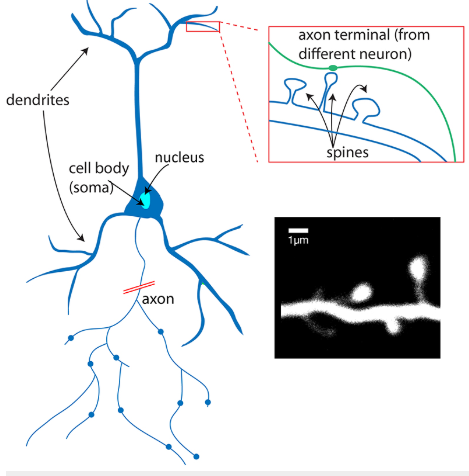
\includegraphics[scale=0.5]{celula-piramidial.png}\\
        {\footnotesize Fonte: The University Of Queensland.}\
        \label{fig:neuronio_biologico}
    \end{figure}
    
    \begin{itemize}
        \item \textbf{Corpo Celular ou Soma: }responsável por integrar os sinais recebidos de outros neurônios;
        \item \textbf{Dendritos: }responsáveis por receber informações transmitidas por outros neurônios. 
        São consideradas as zonas receptivas;
        \item \textbf{Axônio: }responsável por transmitir as informações para outros neurônio também chamadoo de linha de 
        transmissão;
    \end{itemize}

    Quando o conjunto de sinais recebidos é suficientemente forte para ativar o neurônio, este gera um impulso elétrico 
    que percorre seu axônio. Esse sinal eletroquímico coordena e organiza a atividade neuronal, permitindo ao cérebro realizar 
    diversas formas de processamento de maneira extremamente eficiente, muitas vezes mais rápida do que os computadores digitais 
    convencionais~\cite{haykin2009neural}. Ao entender de que forma o cerebro humano processa informações, cientistas buscaram 
    reproduzir seu funcionamento de forma artificial.
    
    Com isso, surgiram as Redes Neurais Artificiais (RNA's), que tenta mimetizar o sistema nervoso humano, RNA's são capazes de
    assimilar e reter conhecimento, possuíndo um alto grau de paralelsimo e extremamente conectada. As RNA's são utilizadas para
    desempenhar a mesma função após o treinamento. Sendo seu elemento constituinte chamado de neurônio artificial~\cite{ulinick2019}.

    De acordo com \citeonline{haykin2009neural}, um neurônio é uma unidade de processamento de informação que é fundamental para a operação de um
    rede neural. Na Figura \ref{fig:fluxo-perceptron} é ilustrado os componentes básicos da arquitetura mais simples de uma rede neural.
    \begin{figure}[!htb]
        \centering
        \caption{Neurônio Artificial (Perceptron).}
        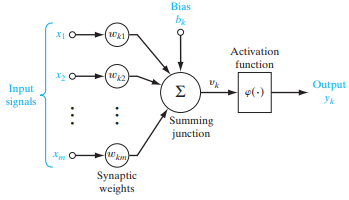
\includegraphics[scale=0.8]{fluxo-perceptron.png}\\
        {\footnotesize Fonte: Haykin (2009).}\
        \label{fig:fluxo-perceptron}
    \end{figure}
    
    \begin{itemize}
        \item \textbf{Entrada: }
        \item \textbf{Sinapses: }
        \item \textbf{Bias: }
        \item \textbf{Somador: }
        \item \textbf{Função de ativação: }
        \item \textbf{Saída: }
    
    \end{itemize}
    % \subsection{Histórico}
    %     As redes neurais são frequentemente consideradas um complemento à computação tradicional. Curiosamente, 
    %     John von Neumann, amplamente reconhecido como o pai da computação moderna devido à sua proposta da arquitetura 
    %     que possibilitou a criação do computador de programa armazenado, demonstrava grande interesse em modelar o 
    %     funcionamento do cérebro humano. Esse interesse levantou debates entre pesquisadores sobre a possível interação 
    %     entre as ideias de von Neumann e os primórdios das redes neurais. Alguns estudiosos destacam indícios que 
    %     sugerem a visão de von Neumann sobre as direções futuras do desenvolvimento dos computadores~\cite{Fausett1994}.

    %     Neste capítulo, serão destacados alguns marcos significativos que tiveram um papel fundamental no avanço e
    %     desenvolvimento da área de redes neurais.

    %     \subsubsection{Perceptrons}
            
    %         Em 1958, o psicólogo Frank Rosenblatt publicou um artigo que, pela primeira vez, descreveu de forma 
    %         algorítmica o funcionamento de um modelo de rede neural para aprendizagem supervisioanda. Essa 
    %         publicação inspirou inúmeros pesquisadores a direcionarem seus esforços para estudos sobre redes neurais, 
    %         explorando diversos aspectos dessa temática ao longo das décadas de 1960 e 1970~\cite{haykin2009neural}.

    %         \begin{figure}[!htb]
    %             \centering
    %             \caption{Fluxo do perceptron.}
    %             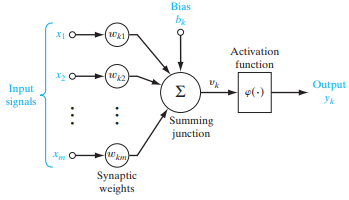
\includegraphics[scale=0.8]{fluxo-perceptron.png}\\
    %             {\footnotesize Fonte: Haykin (2009).}\
    %             \label{fig:fluxo-perceptron}
    %         \end{figure}

    %         Como apresentado na Figura~\ref{fig:fluxo-perceptron}, o perceptron consiste de um único neurônio com 
    %         pesos sinápticos ajustáveis e um viés. Ele possui uma camada de entrada (a retina) conectada aos pesos e 
    %         uma camada de saída. Seu funcionamento baseia-se em um combinador linear seguido por uma função de 
    %         ativação que realiza uma função linear. Esse nó somador (o neurônio) calcula uma combinação linear das 
    %         entradas aplicadas às suas sinapses, além de incorporar um viés aplicado externamente que ajusta a posição
    %         da função de ativação. O resultado dessa soma é passado à função de ativação, que produz uma saída de +1 
    %         se a entrada for positiva, ou -1, se for negativa. 
            
    %         O perceptron é um classificador binário, pois resolve apenas problemas de classificação de padrões 
    %         linearmente separáveis, ou seja, é capaz de lidar exclusivamente com problemas nos quais duas classes 
    %         podem ser separadas por uma linha em um hiperplano~\cite{haykin2009neural}. 


        % \subsubsection{Adaline}

        %     Em 1960, Bernard Widrow e Marcian Hoff desenvolveram uma regra de aprendizagem denominada "Regra Delta", 
        %     também conhecida como Least Mean Squares (LMS) ou método do Gradiente Descendente. Com base nessa regra, 
        %     foi criada uma rede neural com a mesma estrutura do Perceptron, composta por uma camada de entrada, uma 
        %     camada de saída e um único neurônio. A diferença principal reside na regra de aprendizado empregada para 
        %     o ajuste dos pesos, enquanto o Perceptron ajusta os pesos com base na saída binária da rede, essa rede
        %     utiliza a diferença entre o previsto e real e aplica o gradiente descendente para reduzir o erro.
            
        %     A Regra Delta, que tem como finalidade ajustar os pesos do neurônio, busca minimizar a diferença entre a 
        %     saída desejada e a resposta obtida a partir da combinação linear de todas as amostras. Utilizando a 
        %     minimização do erro quadrático médio entre os valores previstos e reais, o método opera dentro de um 
        %     contexto de aprendizagem supervisionada, onde há uma saída esperada previamente definida. O algoritmo 
        %     ajusta iterativamente o vetor de pesos \( w\) atribuído à rede, com o objetivo de determinar um 
        %     \( w^{*} \) ótimo tal que o erro quadrático \({E(w{*})}\), calculado sobre todo o conjunto de amostras, 
        %     seja minimizado.

        %     Essa rede neural foi projetada para aplicações em sistemas de chaveamento de circuitos telefônicos e 
        %     ficou conhecida como Adaline (Adaptive Linear Neuron). A Adaline foi uma das primeiras redes neurais 
        %     implementadas em contextos industriais, marcando um avanço significativo na aplicação de tecnologias 
        %     baseadas em inteligência artificial. Além disso, a regra de aprendizagem Widrow-Hoff para uma rede neural 
        %     de apenas uma camada foi o percursor da regra de Backpropagation para múltiplas camadas~\cite{Fausett1994,silva2010}
                
    \subsection{Processo de Treinamento}
        Sistemas de aprendizado de máquina podem ser categorizados de acordo com o tipo de treinamento que
        eles recebem. O aprendizado supervisionado ocorre quando o modelo é treinado por meio de exemplos explicítos. 
        Em contrapartida, no aprendizado não supervisionado, não há a definição de exemplos explicítos para orientar o 
        modelo. Além disso, existem diversas boas práticas para garantir que o modelo consiga realizar um bom aprendizado 
        e métricas para avalia-lo
         
        \subsubsection{Aprendizado Supervisionado e Não Supervisionado}  
        %Falar de forma breve o que é o aprendizado supervisionado e seus tipos
            No aprendizado supervisionado, o modelo é treinado com pares de dados \((x,y)\), onde \(x\) representa 
            os dados de entrada e \(y\) o valor esperado (ou rótulo). Durante o treinamento, o modelo compara as 
            previsões feitas com os valores reais utilizando uma função de perda, que mede o erro. Em seguida, 
            seus parâmetros são ajustados iterativamente, geralmente por meio de métodos como o gradiente descendente, 
            para minimizar esse erro e melhorar a precisão das previsões.
            
            No aprendizado não supervisionado, o modelo não recebe o par de dados \((x,y)\), mas apenas as entradas 
            \(x\). A partir disso, ele busca identificar padrões, estruturas ou associações presentes nos dados, 
            ajustando os pesos de acordo com o objetivo do método utilizado.

        
        \subsubsection{Pre-Processamento dos Dados}
            Antes de treinar um modelo com algoritmos de aprendizado de máquina, é imprescindível realizar o pré-processamento 
            dos dados. Esse processo assegura que os dados estejam padronizados, consistentes e adequados, permitindo que os 
            modelos alcancem um desempenho superior e resultados confiáveis nas métricas de avaliação. Para isso, são utilizadas 
            técnicas que evitam problemas como dados ausentes, inconsistências, valores conflitantes e incongruentes. Essas 
            técnicas são geralmente divididas em quatro categorias principais: limpeza, integração, transformação e redução de 
            dados~\cite{silva2021, oliveira2024}.

            \subsubsubsection{Limpeza de Dados}
                Um problema comum em conjuntos de dados (\emph{datasets}) é a presença de valores faltantes (ou nulos), que 
                podem ocorrer devido a diferentes fatores. Esses fatores incluem registros manuais realizados de forma 
                inadequada, falhas em sistemas de extração, transformação e carregamento de dados (\emph{ETL}) ou até mesmo 
                problemas em sensores de dispositivos autônomos. A presença de valores faltantes compromete tanto a qualidade 
                dos dados quanto o desempenho do treinamento de modelos de \emph{machine learning}, caso não seja tratada 
                adequadamente.~\citeonline{sivakumar2017} apresentam algumas abordagens eficazes para lidar com essa 
                problemática, como:

                \begin{itemize}
                    \item Exclusão de linhas do \emph{dataset} que contenham valores faltantes.
                    \item Preenchimento dos valores ausentes utilizando métricas estatísticas, como a média ou mediana, 
                    para gerar estimativas aproximadas que mantenham a coerência do conjunto de dados.
                \end{itemize}
                
            \subsubsubsection{Integração de Dados}
                É o processo de combinar dados provenientes de diversas fontes, ecossistemas e tecnologias, de maneira adequada 
                e coerente. Durante esse processo de integração, podem surgir problemas, como inconsistências nos dados e 
                redundâncias no conjunto de dados gerado~\cite{sivakumar2017, silva2021, oliveira2024}.

            \subsubsubsection{Transformação de Dados}
                Nesse estágio, os dados são transformados em formatos adequados para utilização no modelo. 
                \citeonline{sivakumar2017} e \citeonline{oliveira2024} definem algumas atividades executadas nesta 
                etapa:

                \begin{itemize} 
                    \item Uso de normalização para ajustar os valores dos dados a uma escala comum, permitindo fácil comparação entre 
                    diferentes atributos. 
                    \item Eliminação de ruídos com técnicas de suavização. 
                    \item Aplicação de técnicas de agregação para resumir dados complexos e detalhados. 
                    \item Generalização de valores específicos em categorias mais amplas, como, por exemplo, a generalização de 
                    faixas etárias. 
                \end{itemize}

            \subsubsubsection{Redução de Dados}
                Nessa etapa, são utilizadas metodos para reduzir o volume de dados que serão analisados, visando maior velocidade
                de processamento e melhora na eficiência do processo, mas sem comprometer a qualidade e integridade dos dados 
                originais.~\citeonline{sivakumar2017} indicam algumas estrategias, sendo elas:
                \begin{itemize}
                    \item Redução de dimensionalidade do \emph{dataset}, removendo atributos que não melhoram a perfomance do 
                    modelo.
                    \item Utilização de operações de agregação de dados para resumo de informações.
                    \item Utilização de técnicas de \emph{encoding} para compactação de dados.
                \end{itemize}

        \subsubsection{Overfitting e Undefitting}
            Ao construir modelos de redes neurais, diversos desafios podem surgir, sendo dois dos mais comuns o 
            \emph{Overfitting} e o \emph{Underfitting}. O \emph{Overfitting} ocorre quando o modelo aprende tão 
            bem os padrões dos dados de treinamento que sua capacidade de generalização para novos dados é 
            comprometida. Isso acontece porque o modelo não apenas captura as características relevantes dos dados, 
            mas também absorve ruídos e padrões específicos do conjunto de treinamento~\cite{montesinos2022}. 
            Como consequência, ao ser exposto a novos exemplos, seja do conjunto de teste ou de outros conjuntos de 
            dados inéditos, o modelo tende a aplicar regras memorizadas, em vez de identificar padrões generalizáveis. 
            Isso compromete sua capacidade de inferir corretamente a partir de dados não vistos, resultando em um 
            desempenho insatisfatório.

            Por outro lado, o \emph{Underfitting} ocorre quando o modelo é excessivamente simples, muitas vezes 
            devido à utilização de poucas variáveis de entrada. Isso impede que o modelo represente adequadamente 
            os padrões predominantes no \emph{dataset} e capture as características essenciais das amostras, 
            resultando em um desempenho insatisfatório já durante o treinamento. Além disso, esse problema também 
            pode surgir quando o conjunto de dados de treinamento é muito pequeno ou pouco representativo da 
            população, comprometendo ainda mais a capacidade de aprendizagem do modelo~\cite{montesinos2022}.
            
        

        \subsubsection{Técnicas de Validação}
        %Falar o que é, porque foi criada e modo de uso
        \subsubsubsection{Hold-Out}
        \subsubsubsection{K-Fold}
        \subsubsubsection{Leave-One-Out}
        \subsubsubsection{Bootstrap}

        \subsubsection{Métricas de Avaliação}
            Vide que a utilização de modelos de \emph{machine learning} é com o foco de predizer determinados eventos atráves
            de métodos estáticos e probabilisticos. A exatidão da previsão é o fator crucial em avaliar a qualidade de um modelo.
            \citeonline{sousa2011} apresenta a Tabela~\ref{fig:tabela-metricas} com as métricas mais comuns para avaliar as previsões
            dos modelos.
            
            \begin{center}
                \begin{table}[h!]
                    \centering
                    \caption{Métricas de Avaliação}
                    \label{tab:calculo_erros}
                    \begin{tabular}{ll}
                        \toprule
                        \textbf{Designação} & \textbf{Fórmula} \\ 
                        \midrule
                        Erro Absoluto Médio (MAE) & $\frac{1}{n} \sum_{t=1}^{n} |e_t|$ \\[8pt]
                        Erro Quadrático Médio (MSE) & $\frac{1}{n} \sum_{t=1}^{n} (e_t)^2$ \\[8pt]
                        Raiz do Erro Quadrático Médio (RMSE) & $\sqrt{\frac{1}{n} \sum_{t=1}^{n} (e_t)^2}$ \\[8pt]
                        Erro Percentual Absoluto Médio (MAPE) & $\frac{1}{n} \sum_{t=1}^{n} \left(\frac{|e_t|}{|y_t|}\right) 100$ \\ 
                        \bottomrule
                    \end{tabular}
                    
                    \bigskip
                    \small \textbf{Fonte:} Sousa (2011)
                    \label{fig:tabela-metricas}
                \end{table}
            \end{center}
            
            
    \subsection{Multi Layer Perceptron}
    %Falar o que é e botar uma imagem em todas       
        %Colcar uma imagem do mlp detalhada, mostrando os pesos sinapticos, a função de ativação e a backpropagation em ação
        O algoritmo de backpropagation ajusta os pesos da rede neural para reduzir o erro entre a saída prevista 
        e o valor esperado. O erro é calculado e propagado pelas camadas até atingir um nível mínimo aceitável~\cite{marangoni2010}.
        
        \citeonline{grus2021} apresenta o funcionamento padrão do treinamento de uma rede neural utilizando o algoritmo 
        de backpropagation como método de ajuste dos pesos. Considera-se que a rede possui \( n\),  os quais são 
        ajustados de acordo com o seguinte procedimento:
        \begin{enumerate}
            \item Realiza-se o feed-forward, em que as entradas são processadas para produzir as saídas de todos os neurônios;
            \item Como o algoritmo é supervisionado, os valores esperados das saídas são conhecidos. Assim, calcula-se uma função de perda, geralmente definida como a soma dos erros quadráticos entre as saídas reais e as esperadas;
            \item O gradiente dessa função de perda é calculado em relação aos pesos dos neurônios de saída;
            \item Os gradientes e os erros são propagados para trás com o objetivo de calcular os gradientes associados aos pesos dos neurônios ocultos;
            \item Atualizam-se os pesos aplicando um passo em direção ao gradiente descendente, controlado por um parâmetro denominado learning rate (taxa de aprendizagem).
        \end{enumerate}
        % \subsubsection{Redes Neurais Recorrentes}
        %     %Colocar uma imagem de uma RNR, mostrando tudo, detalhando a rede e falar da matemática especifica sobre comoo ela salva o conteudo da camada anterior
        % \subsubsection{Redes Neurais Convolucionais}
        %     %Imagem da arquitetura da rede, como ela opera, o que é a operação de convulação e os outros hiperparametros
        % \subsubsection{Long Short-Term Memory (LSTM)}
        %     %Imagem do LSTM, detalhamento da rede, hiperparametros, como ela funciona e difereça entre ela e a RNC

    \chapter{METODOLOGIA}
%Descrever o desenho da pesquisa

No decorrer deste capítulo são abordados ambiente e metodologia utilizada durante o
desenvolvimento do presente trabalho.

\section{Obtenção dos Dados}

Para a aplicação de modelos de previsão, é essencial dispor de uma quantidade significativa de dados para o 
treinamento, validação e teste do modelo, bem como para a inferência dessas informações sobre a população como um 
todo. No Brasil, o Instituto Nacional de Meteorologia (INMET) é o órgão responsável pelo Banco de Dados 
Meteorológicos (BDMEP), planejado para coletar, armazenar, processar e disponibilizar dados e informações sobre 
variáveis meteorológicas. 

Esses dados podem ser gerados localmente, por meio de estações meteorológicas convencionais ou automáticas, 
ou captados remotamente, utilizando sensores orbitais, radares, entre outros dispositivos~\cite{vianna2017}. 
O Banco de Dados Meteorológicos para Ensino e Pesquisa (BDMEP), em particular, reúne informações meteorológicas 
diárias provenientes das estações da rede do INMET, seguindo as normas técnicas da Organização Meteorológica 
Mundial (INMET, s.d.).

% O presente trabalhou utilizou os dados da estação meterológica autmática 
\section{Preparação dos Dados}
    \chapter{RESULTADOS ESPERADOS}
    Espera-se que o modelo baseado em redes neurais artificiais consiga prever as oscilações na 
    temperatura média do município de Itapetinga-BA com um nível satisfatório de precisão. Além disso, 
    busca-se identificar padrões na série temporal estudada, proporcionando uma compreensão mais detalhada 
    das dinâmicas climáticas locais. Os resultados obtidos deste trabalho poderão contribuir para pesquisas 
    futuras sobre as alterações do clima na região.
    \chapter{Cronograma}

\begin{table}[h]
    \centering
    \footnotesize
    \renewcommand{\arraystretch}{1}
    
    \resizebox{0.9\linewidth}{!}{ % Ajusta automaticamente
        \begin{tabular}{lcccccc}
            \toprule
            \textbf{Etapas} & \textbf{Out/2024} & \textbf{Nov/2024} & \textbf{Dez/2024} & \textbf{Jan/2025} & \textbf{Fev/2025} & \textbf{Mar/2025} \\ 
            \midrule
            Escolha do tema & x &  &  &  &  &  \\ 
            Levantamento biblio. & x &  &  &  &  &  \\ 
            Elab. do anteprojeto &  & x &  &  &  &  \\ 
            Apres. do projeto &  &  & x &  &  &  \\ 
            Desenvolvimento &  &  &  & x & x & x \\ 
            Org. do roteiro & x &  &  &  &  &  \\ 
            Redação &  &  &  &  & x &  \\ 
            Revisão final &  &  &  &  & x & x \\ 
            Entrega &  &  &  &  & x & x \\ 
            \bottomrule
        \end{tabular}
    }
    
    \caption{Cronograma de desenvolvimento do trabalho}
    \label{tab:cronograma}
\end{table}



    % \chapter{CONSIDERAÇÕES FINAIS}

    % Referências
    \nocite{ipcc2020climate}
    \bibliography{referencias}

\end{document}
